\documentclass[11pt,a4paper]{article}
\usepackage[margin=1in]{geometry}
\usepackage{amsmath,amssymb,booktabs,graphicx,hyperref,enumitem,float}
\usepackage{fancyhdr}
\pagestyle{fancy}
\fancyhf{}
\lhead{AI651 Assignment 1}
\rhead{Fall 2026}
\cfoot{\thepage}
\setlength{\parskip}{0.45em}
\setlength{\parindent}{0pt}
\graphicspath{{Question 1/results/design/}}

\title{Assignment 1 Report\\[0.2em]\large AI651 --- Deep Learning for Space, Time and Graphs}
\author{}
\date{Fall 2026}

\begin{document}
\maketitle

\noindent
\textbf{GitHub (public):} \texttt{https://github.com/junaid074/AI651-PA1}

\vspace{0.3em}
\noindent
Task 1 notebook: \texttt{Question 1/Assignment1.ipynb} (full preset, seed 0)\\
Task 2 code: \texttt{Question 2 - Leaderboard/src/train\_leaderboard.py}\\
Forecast paste: \texttt{Question 2 - Leaderboard/outputs/leaderboard\_predictions.txt}\\
Current board declarations: $P{=}32586$, $E{=}20$ (attempt 4)

\section{Task 1}

\subsection{Response 1A}

I expected period-routed ridge to win on both established stations and Station~4, then Raw Attention, then the two plain ridge models. Sensor-specific ridge should fail on Station~4 because that sensor never gets its own matrix.

Validation RMSE (m/s$^2$), full preset:

\begin{center}
\begin{tabular}{lcc}
\toprule
 & Established & Station 4 \\
\midrule
Shared ridge & 0.767 & 0.876 \\
Sensor-specific & 0.768 & n/a \\
Period-routed & 0.166 & 0.173 \\
Raw Attention & 0.424 & 0.617 \\
\bottomrule
\end{tabular}
\end{center}

That is the order I guessed, just more one-sided. Shared and sensor-specific are almost the same on established stations, so the issue is not ``which sensor'' --- it is ``what pace is this run on''. Attention can change the mix per window, so it beats a single shared map, but it still loses to a model that is given the period band. Products A/B/C tell the same story: period-routed stays near 0.15--0.18.

\subsection{Response 1B}

Output~1.2 is one station on a fast Product~A run and a slow Product~C run. One shared $\widehat W$ cannot follow both. Least squares splits the difference, so peaks land late or early on at least one pace.

\begin{figure}[H]
\centering
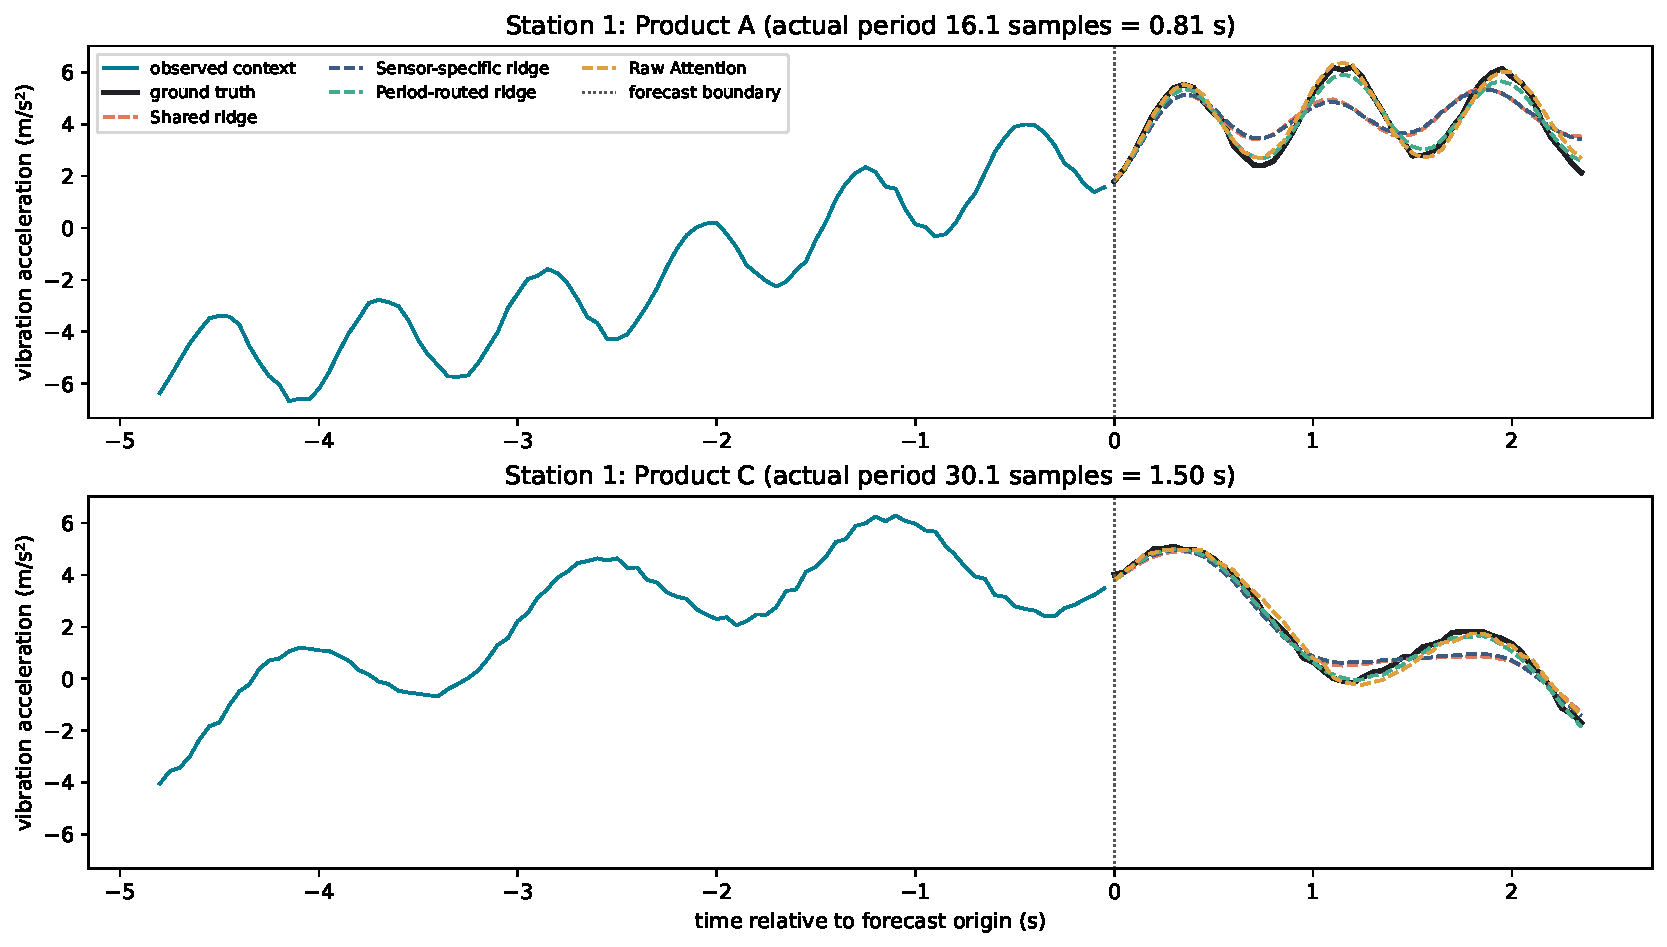
\includegraphics[width=0.95\textwidth]{1.2-1.pdf}
\caption{Output 1.2 --- same station, two paces.}
\end{figure}

Output~1.3 uses the same $W_Q,W_K,W_V$, but the weights move when the context moves. Ridge never does that. I am not saying Attention recovered the physical period --- only that the mix depends on the window.

\begin{figure}[H]
\centering
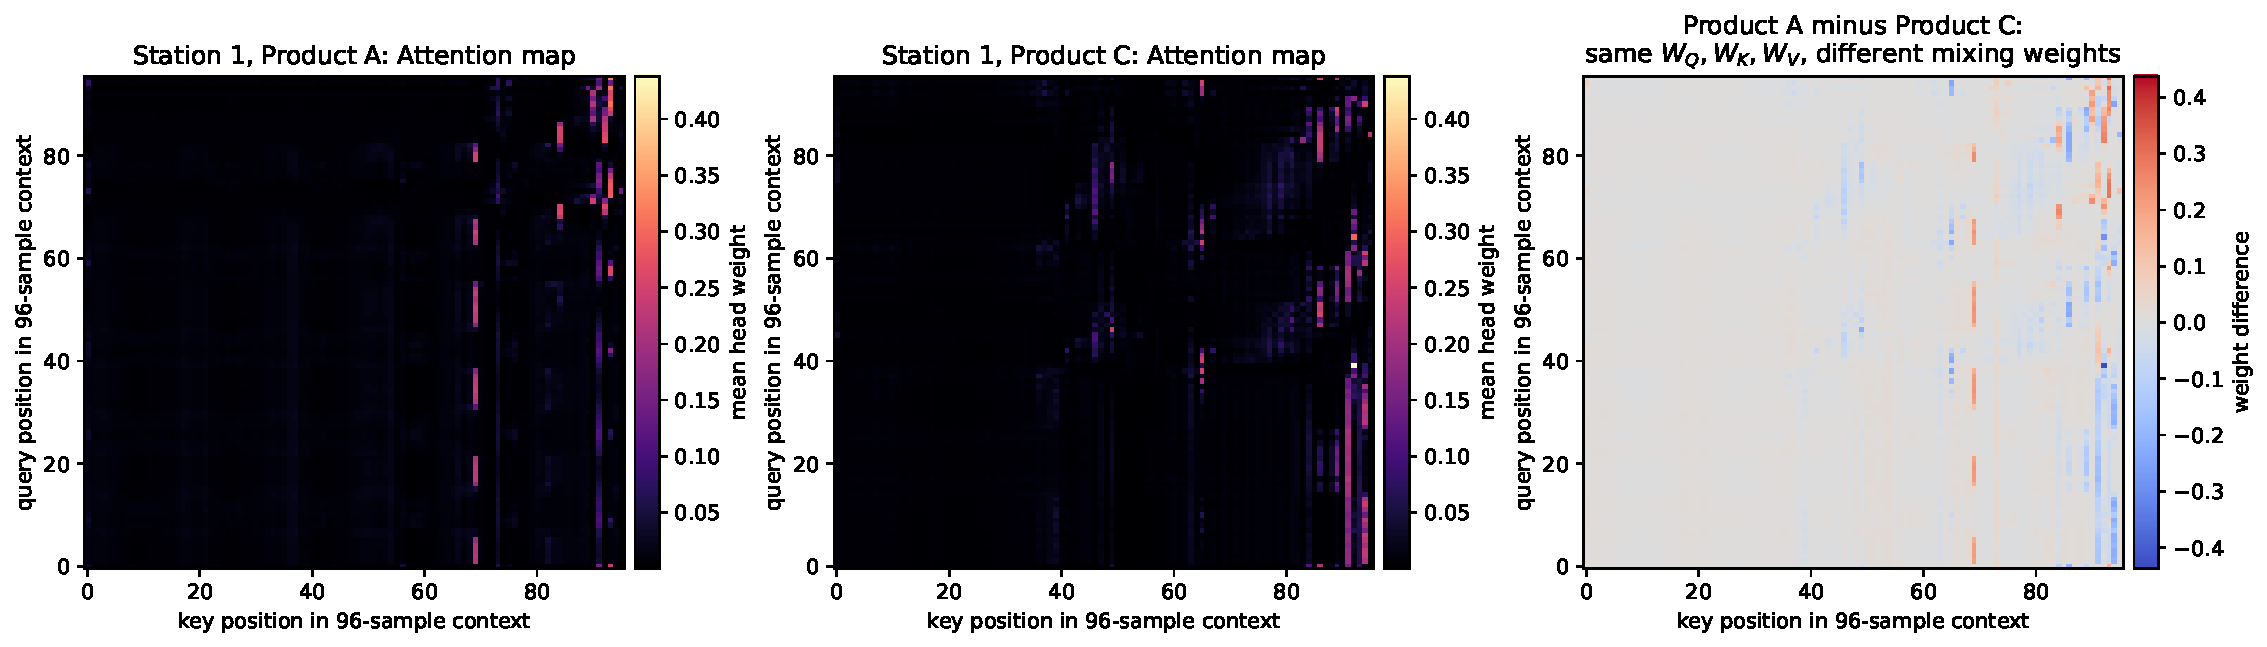
\includegraphics[width=0.95\textwidth]{1.3-1.pdf}
\caption{Output 1.3 --- Attention weights change with the input.}
\end{figure}

\subsection{Response 2}

I implemented a centered moving average with replicate padding at the ends (zeros pull the edges down and fail the check). Return order is (remainder, trend) so $S+T=x$.

Width $m=41$ came from Output~2.2 (best oracle period recovery on training). In Output~2.1, a wider kernel puts more of the slow ramp into $T$. Width 41 is still small next to the ~240-sample drift, but large enough versus the 14--36 sample vibration.

\begin{figure}[H]
\centering
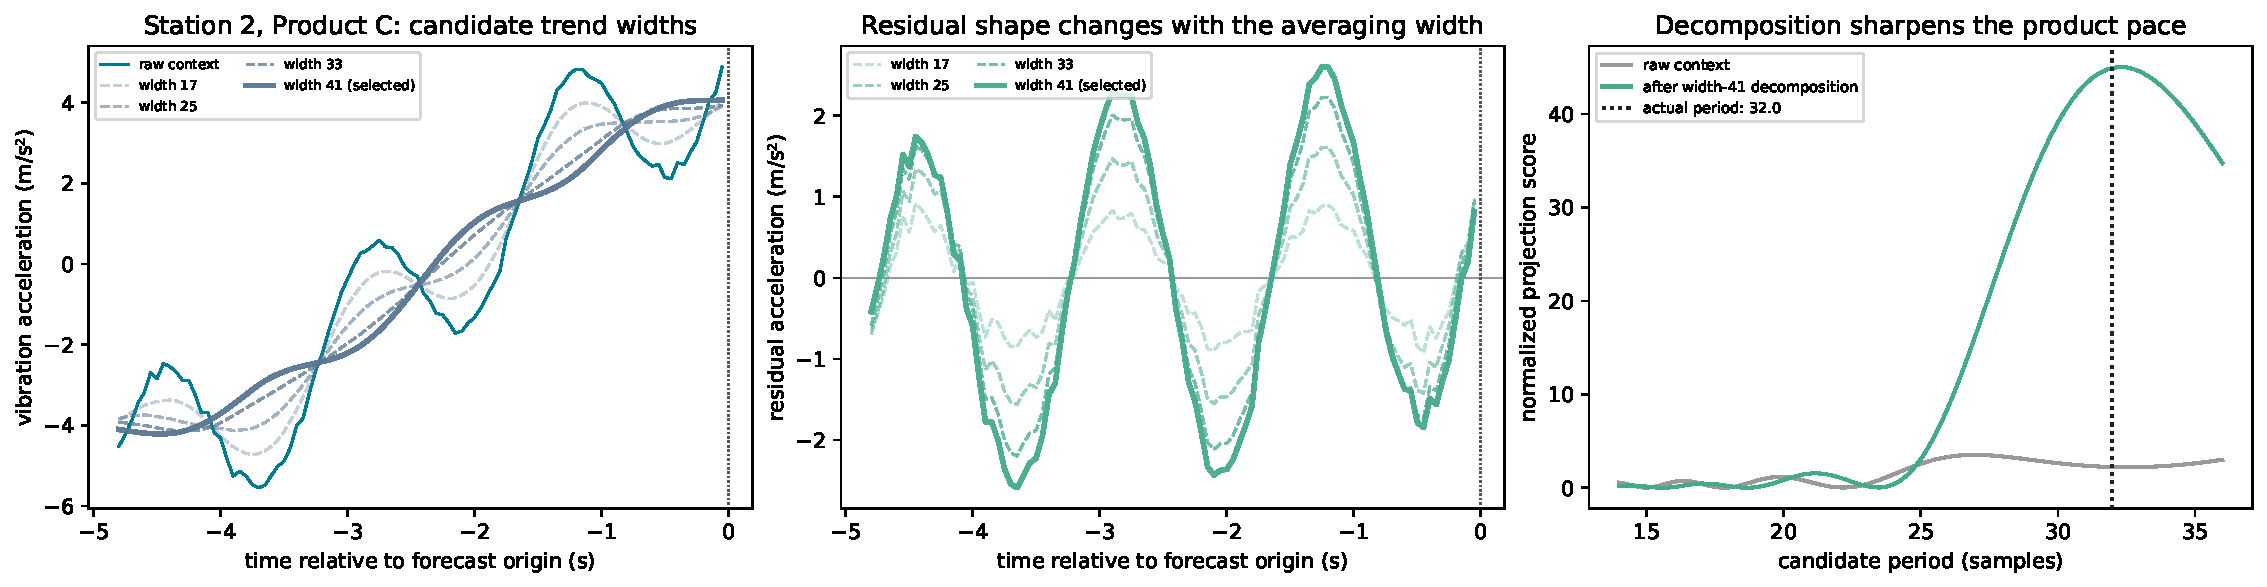
\includegraphics[width=0.95\textwidth]{2.1-1.pdf}
\caption{Output 2.1 --- different widths.}
\end{figure}

\begin{figure}[H]
\centering
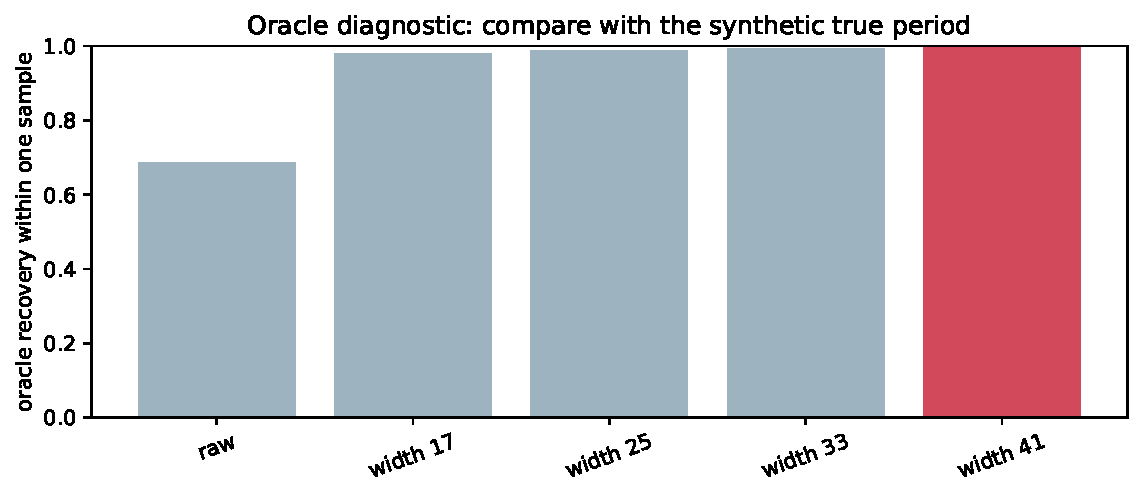
\includegraphics[width=0.75\textwidth]{2.2-1.pdf}
\caption{Output 2.2 --- oracle used to pick $m=41$.}
\end{figure}

Raw Attention validation RMSE: 0.424 / 0.617 (established / held-out). With decomposition: 0.293 / 0.436. Splitting helps.

\begin{figure}[H]
\centering
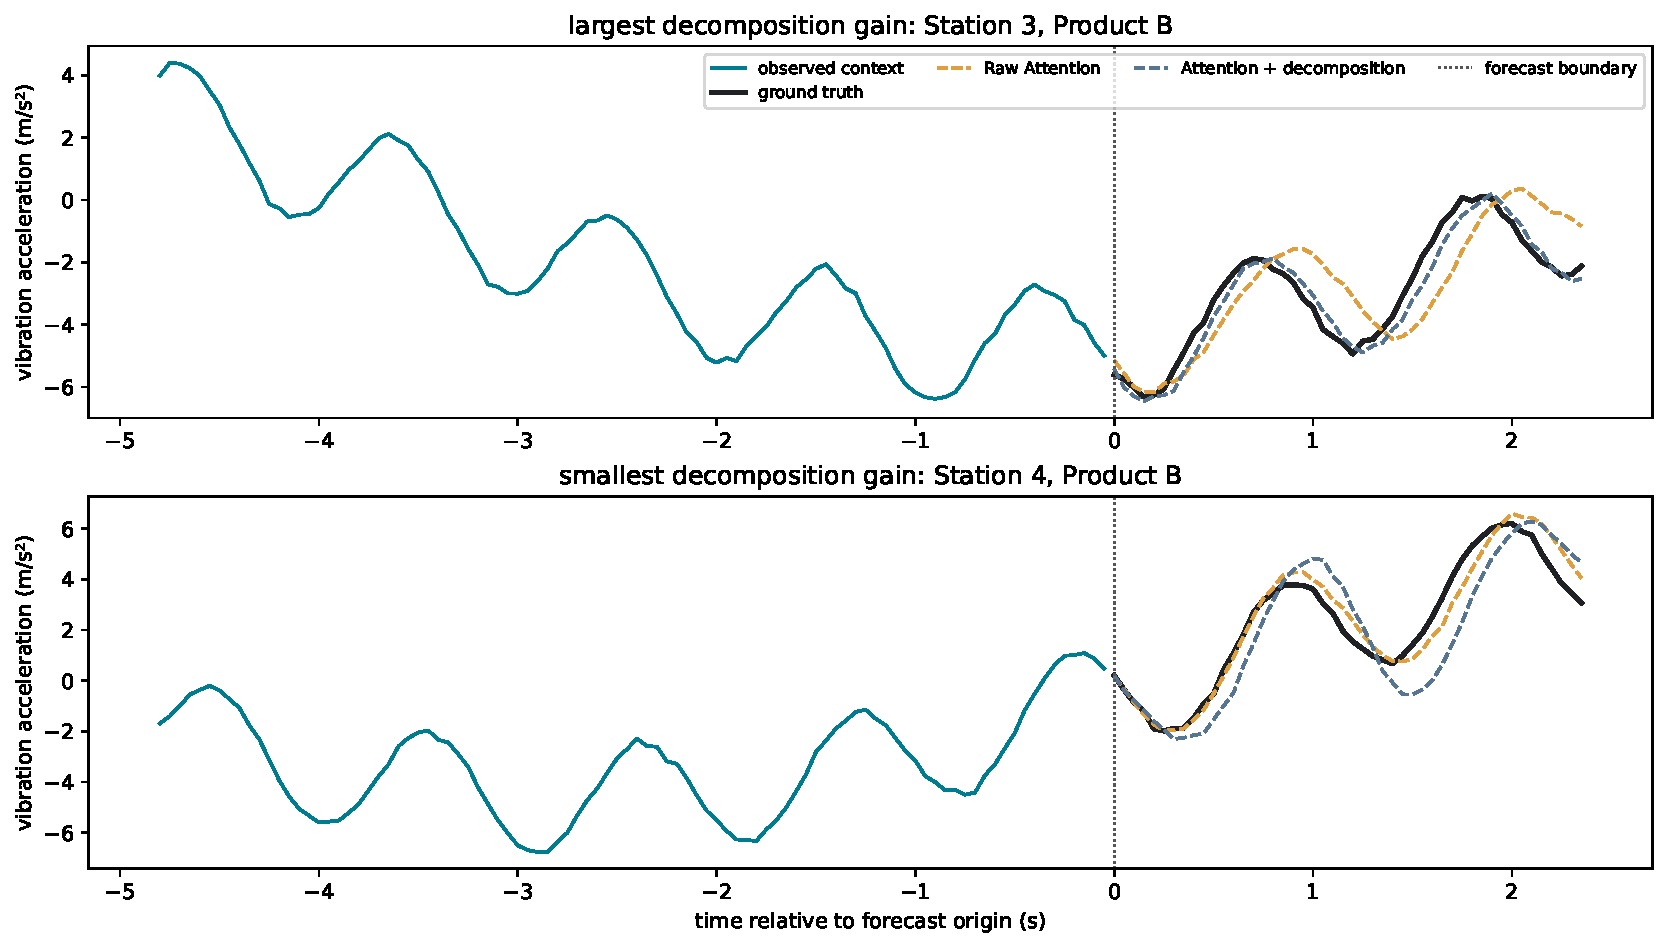
\includegraphics[width=0.95\textwidth]{2.3-1.pdf}
\caption{Output 2.3 --- Attention with vs without decomposition.}
\end{figure}

Why a moving average fits this data: over one 96-sample context the slow part is smooth, and the cycle sits on top of it. After subtracting $T$, the mixer mostly sees vibration. The oracle is only for choosing $m$; the model never sees true $s_i(t)$.

This bias fails on a sharp jump inside the window --- the jump gets smeared into the trend and then leaks into the residual. First differences would treat ``trend'' as local change, not local mean.

\subsection{Response 3}

\texttt{aggregate\_delays}:
\[
z_t = \sum_{j=1}^{K} \alpha_j\, v_{(t-\tau_j)\bmod L}.
\]
I used gather so it stays differentiable. The notebook toy needs $z_0=35$; rolling the wrong way gives 25.

Output~3.1 matches the hand calculation. Output~3.2 is a signal check, not the trained mixer scores. After the slow part is removed, correlation peaks near $P$ and $2P$ (delays 16 and 32 on the plotted run, residual corr $\approx 0.98$). On the raw line the ramp looks similar under many shifts, so the period is harder to see. Delay mixing wants a residual stream.

\begin{figure}[H]
\centering
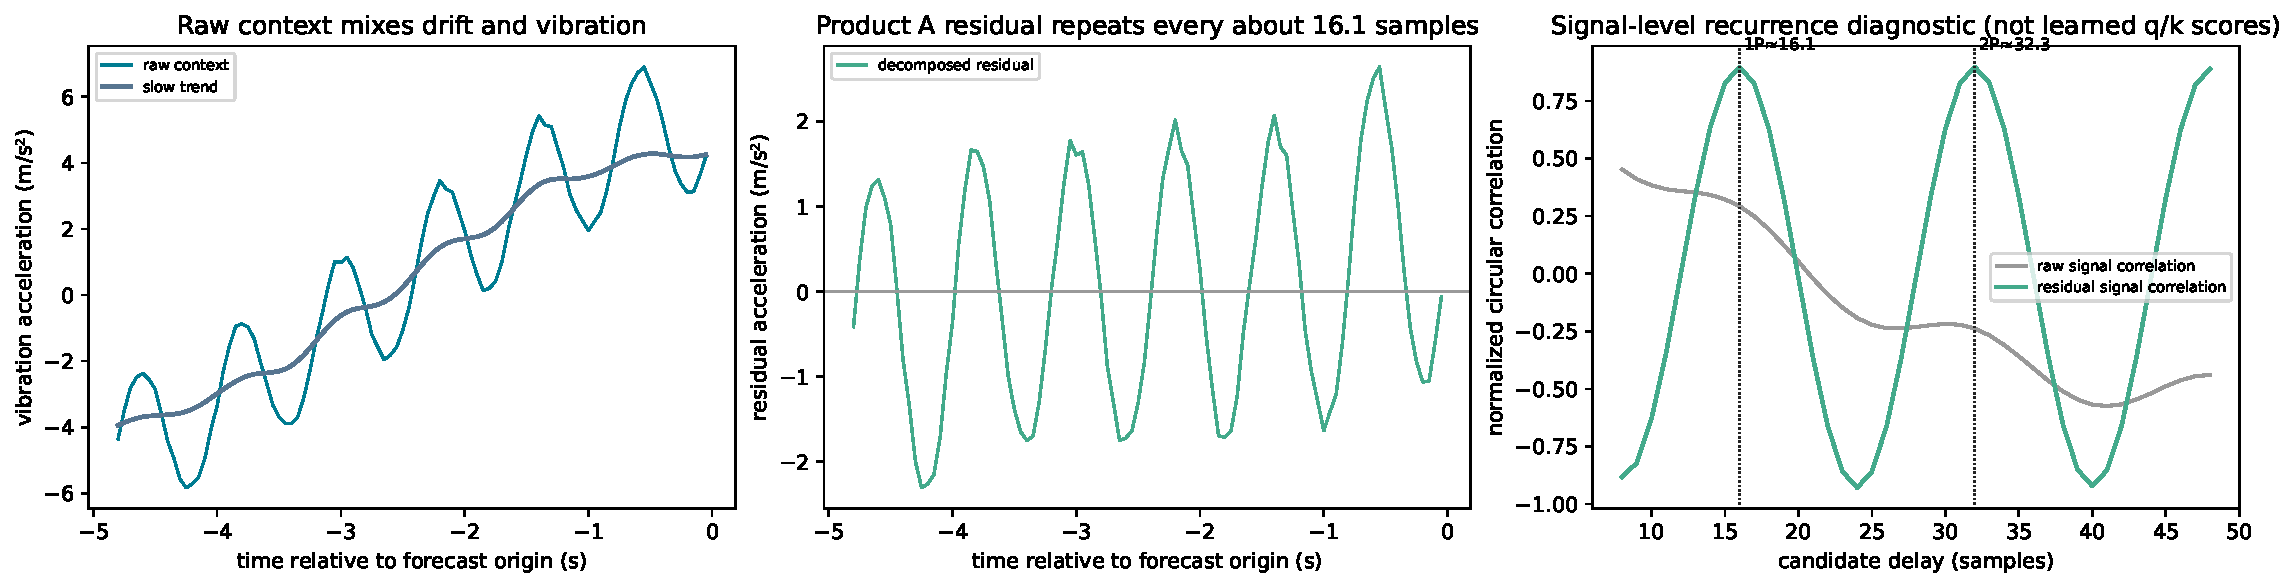
\includegraphics[width=0.95\textwidth]{3.2-1.pdf}
\caption{Output 3.2 --- recurrence on raw vs residual.}
\end{figure}

Bad case: a one-off spike, or the period changing inside the same 96-sample context. Then there is no single ``best delay''.

\subsection{Response 4}

(a) Before Output~4.1 I thought decomposition would matter most when the slow ramp is large, because otherwise Attention spends capacity on the baseline.

(b) Established validation:

\begin{center}
\small
\begin{tabular}{lrrrr}
\toprule
Model & RMSE & MSE & \#params & fit (s) \\
\midrule
Shared ridge & 0.767 & 0.588 & 4.6k & $\approx$0 \\
Sensor-specific & 0.768 & 0.590 & 13.8k & $\approx$0 \\
Period-routed & 0.166 & 0.028 & 59.9k & $\approx$0 \\
Raw Attention & 0.424 & 0.180 & 368k & 418 \\
Attn + decomp & 0.293 & 0.086 & 373k & 557 \\
Raw delay & 0.226 & 0.051 & 368k & 509 \\
Autoformer-style & 0.199 & 0.039 & 373k & 570 \\
\bottomrule
\end{tabular}
\end{center}

Held-out RMSE: period-routed 0.173, Autoformer-style 0.244, raw delay 0.332, attn+decomp 0.436, raw attn 0.617.

\begin{figure}[H]
\centering
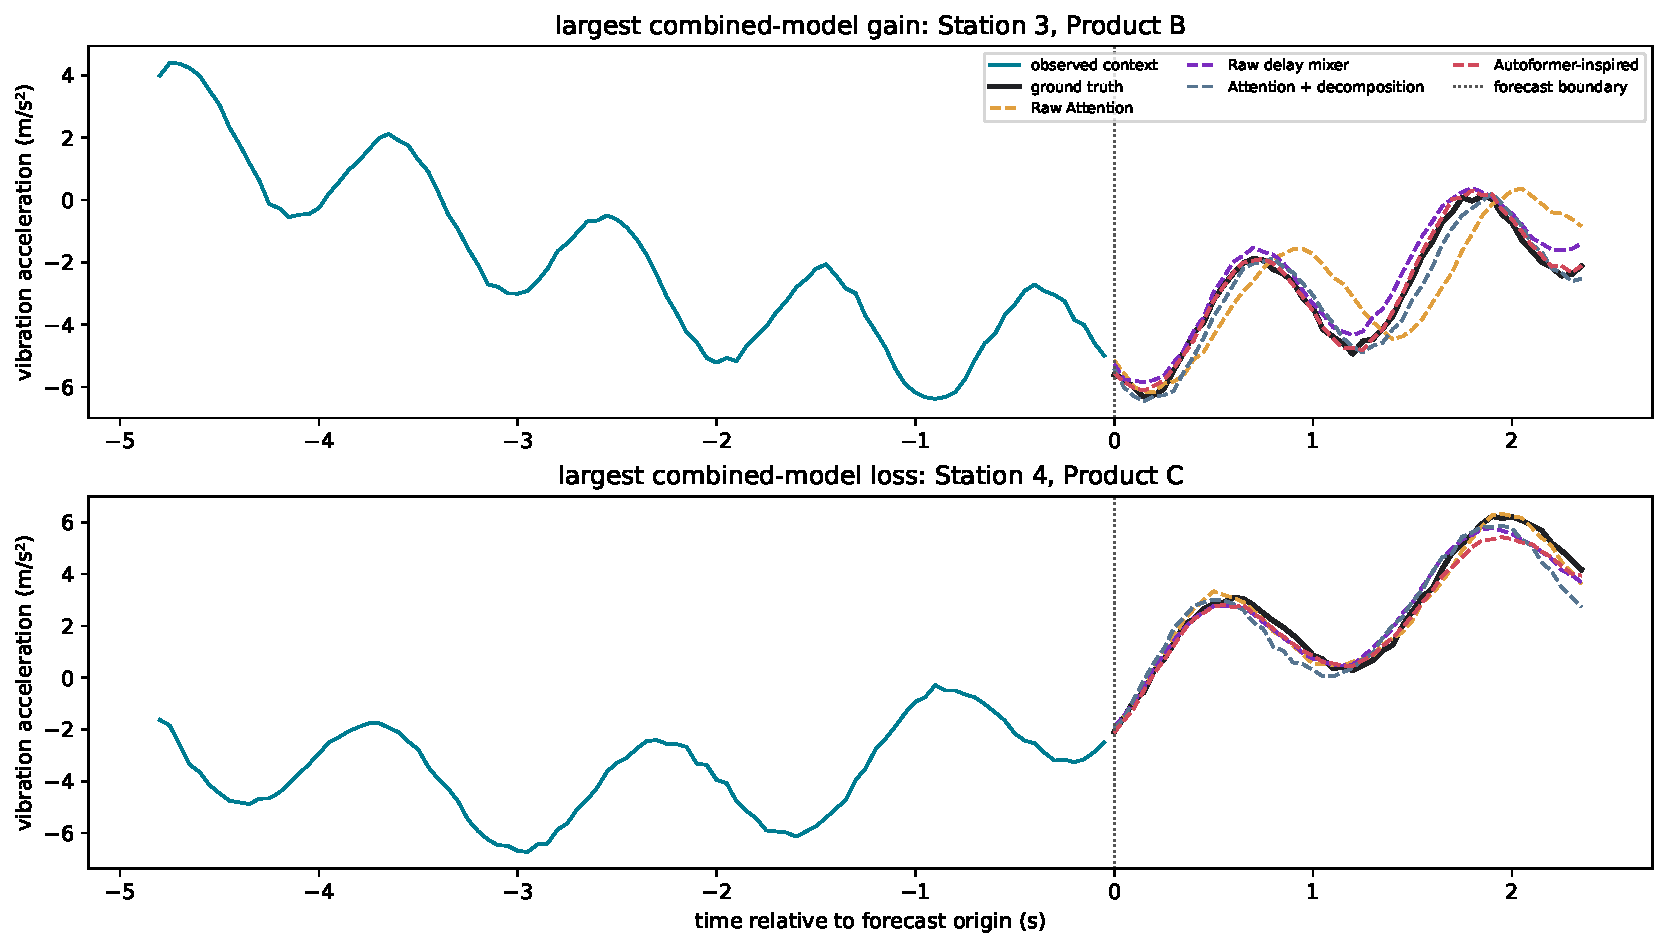
\includegraphics[width=0.95\textwidth]{4.1-1.pdf}
\caption{Output 4.1 --- four neural setups.}
\end{figure}

\begin{figure}[H]
\centering
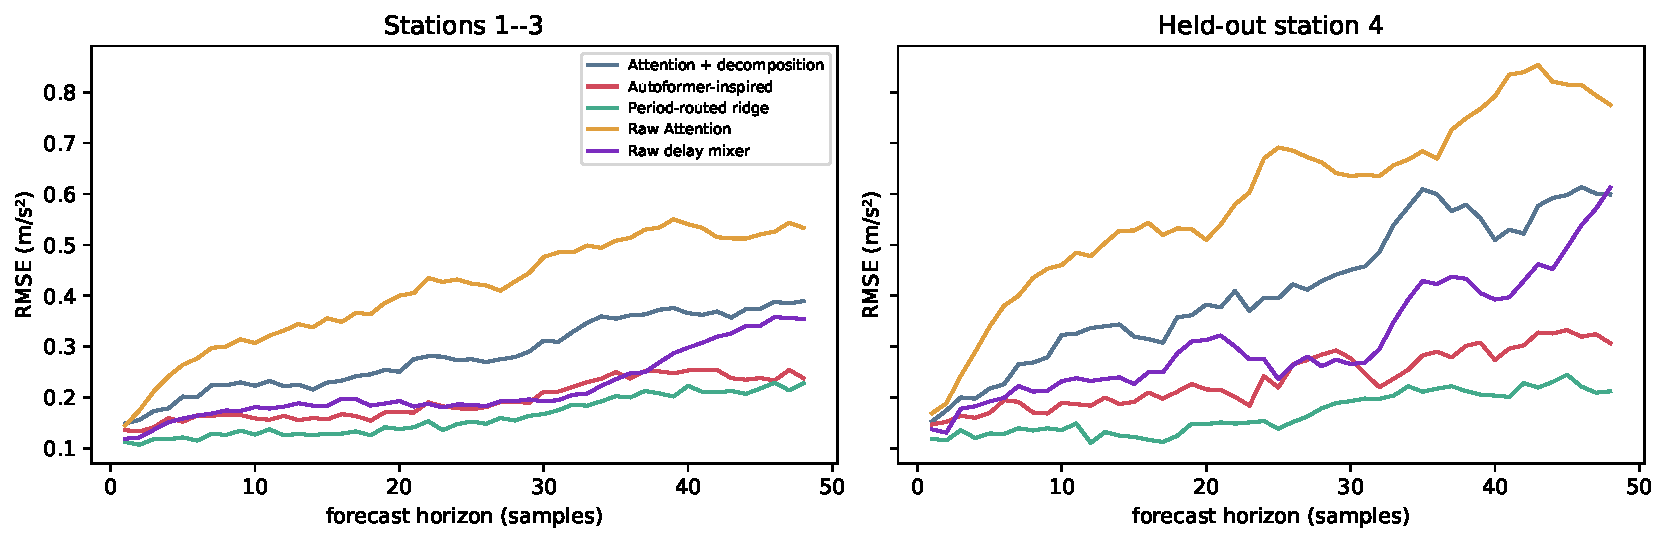
\includegraphics[width=0.95\textwidth]{4.2-1.pdf}
\caption{Output 4.2 --- error vs horizon.}
\end{figure}

Both switches help. Delay mixing alone beats decomp alone. Using both is the best neural option, but the combined gain is less than adding the two separate gains --- they attack related problems. Errors grow with the horizon; period routing stays lowest throughout.

(c) I deploy \textbf{period-routed ridge} for established stations and for Station~4. Best validation error, cheap to fit, and it still works on the held-out sensor. Autoformer-style is the neural winner but worse and slower. Test RMSE: 0.161 (established), 0.183 (Station~4).

Takeaway: naming the right variable (pace) beat a bigger flexible model here.

\section{Task 2}

The submitted model is Autoformer: moving-average decomposition plus auto-correlation / delay aggregation, $\mathrm{pred\_len}=168$. Decomp and delay gather follow the same idea as Question~1. Extra pieces I added: $\log(1+y)$, per-window mean/std on the target, $L=336$, label length 84, AdamW + OneCycle, and a small linear head on the last 8 values (lag-1 is strong on this series).

I also feed the optional covariate file into both encoder and decoder (future values over the horizon are in that file). From \texttt{time\_idx} I built hour-of-day and day-of-week sin/cos. There is no calendar column, but the index is hourly and those cycles showed up in simple checks.

Validation = last several non-overlapping 168-step blocks. After attempts 1--3 scored ~115--120 on the board, I also held out the last training week once as a proxy, because the earlier val score was too kind.

\subsection{Optional file ablation}

Same small setup, chronological val RMSE:

\begin{center}
\begin{tabular}{lcc}
\toprule
 & seed 0 & seed 1 \\
\midrule
target only & 106.06 & 108.70 \\
+ optional file & 73.20 & 81.02 \\
\bottomrule
\end{tabular}
\end{center}

The optional file helps on both seeds. Feature\_D and feature\_H were among the stronger raw correlations. The submitted run keeps that file plus the index-based hour/dow features.

\subsection{Leaderboard attempts}

\begin{center}
\small
\begin{tabular}{ccccp{5.6cm}}
\toprule
Att. & $P$ & $E$ & Board RMSE & What I sent \\
\midrule
1 & 32330 & 12 & $\approx$120.47 & first Autoformer, covariates, no calendar \\
2 & 7530 & 15 & --- & much smaller net; local val looked good \\
3 & 7530 & 15 & 114.59 & MAE 74.58, sMAPE 66.82\% (best on the site so far) \\
4 & 32586 & 20 & (this paste) & 2 encoder layers + hour/dow features \\
\bottomrule
\end{tabular}
\end{center}

Attempts 1--3 all landed near 115--120. Shrinking the net (attempt 2/3) barely moved the board. The local val I had used was leaking (refit on val blocks) and had no calendar features, so it was not a good stand-in for the hidden week.

Attempt 4 is the file in \texttt{leaderboard\_predictions.txt}. Same Autoformer, $d_{\mathrm{model}}{=}32$, 2 encoder layers, optional covariates, hour/dow features, 18 training epochs plus a 2-epoch refit ($E{=}20$). On a last-week holdout inside the training file this setup was much closer to the recent level (proxy RMSE $\approx 37$ on seed 0, $\approx 41$ on seed 1). That is still only a local check --- the board week can differ --- but it is why I am sending this one rather than another 7k-parameter run.

\section*{AI tools}

I used a chat assistant for the Task~2 Autoformer wiring and for running / checking training jobs.

\begin{itemize}[leftmargin=1.2em,itemsep=0.15em]
\item \textbf{Prompt (rough):} help set up an Autoformer encoder--decoder for a 168-step forecast with series decomposition and auto-correlation, plus a training loop on the student CSV.
\item \textbf{What it gave:} a skeleton model and train script.
\item \textbf{What I changed:} delay gather direction after the notebook check, sinusoidal PE, the small level head, width $m$ and the ridge deployment from my full-preset tables, and covariates / hour-dow from my own ablations.
\end{itemize}

\end{document}
